% Created by tikzDevice version 0.12.6 on 2026-04-27 14:13:34
% !TEX encoding = UTF-8 Unicode
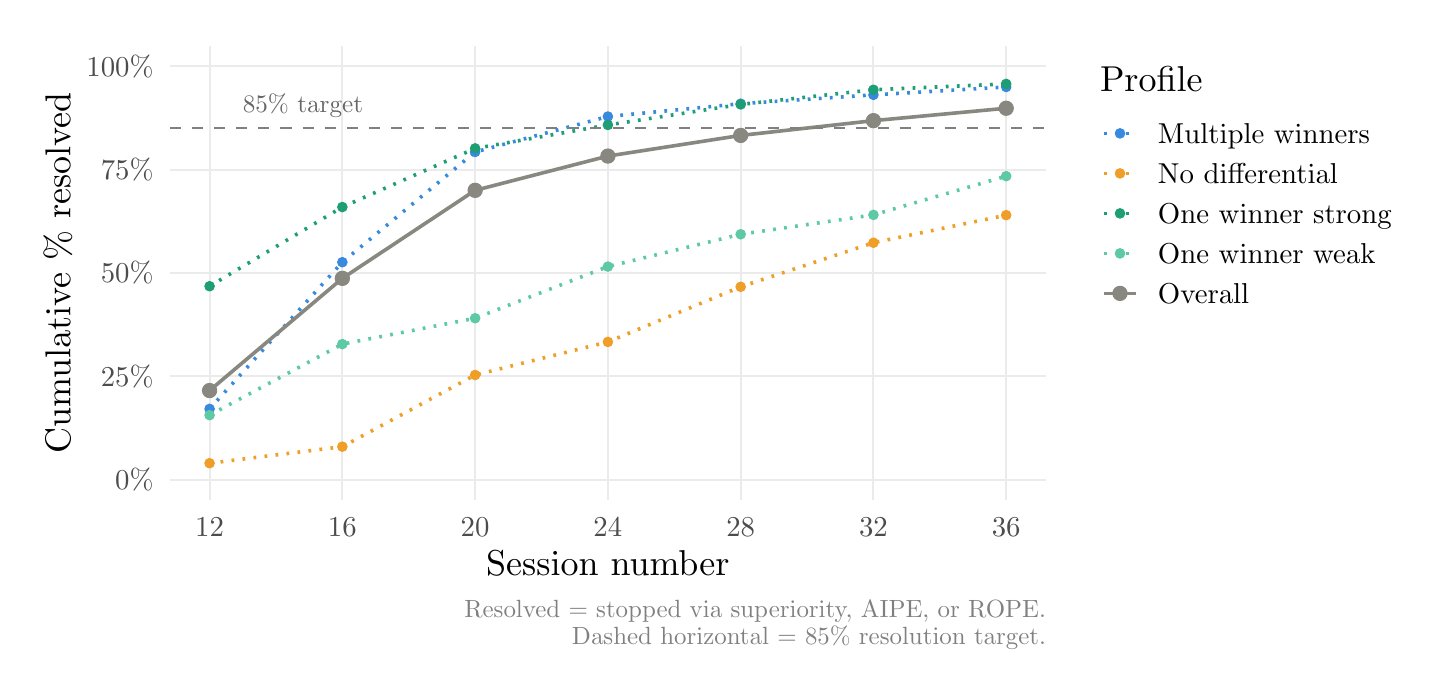
\begin{tikzpicture}[x=1pt,y=1pt]
\definecolor{fillColor}{RGB}{255,255,255}
\path[use as bounding box,fill=fillColor,fill opacity=0.00] (0,0) rectangle (505.89,231.26);
\begin{scope}
\path[clip] (  0.00,  0.00) rectangle (505.89,231.26);
\definecolor{fillColor}{RGB}{255,255,255}

\path[fill=fillColor] ( -0.00,  0.00) rectangle (505.89,231.26);
\end{scope}
\begin{scope}
\path[clip] ( 51.34, 60.43) rectangle (367.99,224.76);
\definecolor{drawColor}{gray}{0.92}

\path[draw=drawColor,line width= 0.7pt,line join=round] ( 51.34, 67.90) --
	(367.99, 67.90);

\path[draw=drawColor,line width= 0.7pt,line join=round] ( 51.34,105.25) --
	(367.99,105.25);

\path[draw=drawColor,line width= 0.7pt,line join=round] ( 51.34,142.60) --
	(367.99,142.60);

\path[draw=drawColor,line width= 0.7pt,line join=round] ( 51.34,179.95) --
	(367.99,179.95);

\path[draw=drawColor,line width= 0.7pt,line join=round] ( 51.34,217.29) --
	(367.99,217.29);

\path[draw=drawColor,line width= 0.7pt,line join=round] ( 65.73, 60.43) --
	( 65.73,224.76);

\path[draw=drawColor,line width= 0.7pt,line join=round] (113.71, 60.43) --
	(113.71,224.76);

\path[draw=drawColor,line width= 0.7pt,line join=round] (161.69, 60.43) --
	(161.69,224.76);

\path[draw=drawColor,line width= 0.7pt,line join=round] (209.66, 60.43) --
	(209.66,224.76);

\path[draw=drawColor,line width= 0.7pt,line join=round] (257.64, 60.43) --
	(257.64,224.76);

\path[draw=drawColor,line width= 0.7pt,line join=round] (305.62, 60.43) --
	(305.62,224.76);

\path[draw=drawColor,line width= 0.7pt,line join=round] (353.59, 60.43) --
	(353.59,224.76);
\definecolor{drawColor}{RGB}{55,138,221}

\path[draw=drawColor,line width= 1.3pt,dash pattern=on 1pt off 3pt ,line join=round] ( 65.73, 93.51) --
	(113.71,146.51) --
	(161.69,186.35) --
	(209.66,199.15) --
	(257.64,203.78) --
	(305.62,206.98) --
	(353.59,209.82);
\definecolor{drawColor}{RGB}{239,159,39}

\path[draw=drawColor,line width= 1.3pt,dash pattern=on 1pt off 3pt ,line join=round] ( 65.73, 73.88) --
	(113.71, 79.85) --
	(161.69,105.75) --
	(209.66,117.70) --
	(257.64,137.62) --
	(305.62,153.55) --
	(353.59,163.51);
\definecolor{drawColor}{RGB}{29,158,117}

\path[draw=drawColor,line width= 1.3pt,dash pattern=on 1pt off 3pt ,line join=round] ( 65.73,137.83) --
	(113.71,166.44) --
	(161.69,187.63) --
	(209.66,196.10) --
	(257.64,203.52) --
	(305.62,208.82) --
	(353.59,210.94);
\definecolor{drawColor}{RGB}{93,202,165}

\path[draw=drawColor,line width= 1.3pt,dash pattern=on 1pt off 3pt ,line join=round] ( 65.73, 91.24) --
	(113.71,116.92) --
	(161.69,126.26) --
	(209.66,144.93) --
	(257.64,156.60) --
	(305.62,163.61) --
	(353.59,177.61);
\definecolor{drawColor}{RGB}{136,135,128}

\path[draw=drawColor,line width= 1.3pt,line join=round] ( 65.73,100.13) --
	(113.71,140.68) --
	(161.69,172.48) --
	(209.66,184.86) --
	(257.64,192.32) --
	(305.62,197.66) --
	(353.59,202.14);
\definecolor{drawColor}{RGB}{55,138,221}
\definecolor{fillColor}{RGB}{55,138,221}

\path[draw=drawColor,line width= 0.4pt,line join=round,line cap=round,fill=fillColor] ( 65.73, 93.51) circle (  1.71);
\definecolor{drawColor}{RGB}{239,159,39}
\definecolor{fillColor}{RGB}{239,159,39}

\path[draw=drawColor,line width= 0.4pt,line join=round,line cap=round,fill=fillColor] ( 65.73, 73.88) circle (  1.71);
\definecolor{drawColor}{RGB}{29,158,117}
\definecolor{fillColor}{RGB}{29,158,117}

\path[draw=drawColor,line width= 0.4pt,line join=round,line cap=round,fill=fillColor] ( 65.73,137.83) circle (  1.71);
\definecolor{drawColor}{RGB}{93,202,165}
\definecolor{fillColor}{RGB}{93,202,165}

\path[draw=drawColor,line width= 0.4pt,line join=round,line cap=round,fill=fillColor] ( 65.73, 91.24) circle (  1.71);
\definecolor{drawColor}{RGB}{55,138,221}
\definecolor{fillColor}{RGB}{55,138,221}

\path[draw=drawColor,line width= 0.4pt,line join=round,line cap=round,fill=fillColor] (113.71,146.51) circle (  1.71);
\definecolor{drawColor}{RGB}{239,159,39}
\definecolor{fillColor}{RGB}{239,159,39}

\path[draw=drawColor,line width= 0.4pt,line join=round,line cap=round,fill=fillColor] (113.71, 79.85) circle (  1.71);
\definecolor{drawColor}{RGB}{29,158,117}
\definecolor{fillColor}{RGB}{29,158,117}

\path[draw=drawColor,line width= 0.4pt,line join=round,line cap=round,fill=fillColor] (113.71,166.44) circle (  1.71);
\definecolor{drawColor}{RGB}{93,202,165}
\definecolor{fillColor}{RGB}{93,202,165}

\path[draw=drawColor,line width= 0.4pt,line join=round,line cap=round,fill=fillColor] (113.71,116.92) circle (  1.71);
\definecolor{drawColor}{RGB}{55,138,221}
\definecolor{fillColor}{RGB}{55,138,221}

\path[draw=drawColor,line width= 0.4pt,line join=round,line cap=round,fill=fillColor] (161.69,186.35) circle (  1.71);
\definecolor{drawColor}{RGB}{239,159,39}
\definecolor{fillColor}{RGB}{239,159,39}

\path[draw=drawColor,line width= 0.4pt,line join=round,line cap=round,fill=fillColor] (161.69,105.75) circle (  1.71);
\definecolor{drawColor}{RGB}{29,158,117}
\definecolor{fillColor}{RGB}{29,158,117}

\path[draw=drawColor,line width= 0.4pt,line join=round,line cap=round,fill=fillColor] (161.69,187.63) circle (  1.71);
\definecolor{drawColor}{RGB}{93,202,165}
\definecolor{fillColor}{RGB}{93,202,165}

\path[draw=drawColor,line width= 0.4pt,line join=round,line cap=round,fill=fillColor] (161.69,126.26) circle (  1.71);
\definecolor{drawColor}{RGB}{55,138,221}
\definecolor{fillColor}{RGB}{55,138,221}

\path[draw=drawColor,line width= 0.4pt,line join=round,line cap=round,fill=fillColor] (209.66,199.15) circle (  1.71);
\definecolor{drawColor}{RGB}{239,159,39}
\definecolor{fillColor}{RGB}{239,159,39}

\path[draw=drawColor,line width= 0.4pt,line join=round,line cap=round,fill=fillColor] (209.66,117.70) circle (  1.71);
\definecolor{drawColor}{RGB}{29,158,117}
\definecolor{fillColor}{RGB}{29,158,117}

\path[draw=drawColor,line width= 0.4pt,line join=round,line cap=round,fill=fillColor] (209.66,196.10) circle (  1.71);
\definecolor{drawColor}{RGB}{93,202,165}
\definecolor{fillColor}{RGB}{93,202,165}

\path[draw=drawColor,line width= 0.4pt,line join=round,line cap=round,fill=fillColor] (209.66,144.93) circle (  1.71);
\definecolor{drawColor}{RGB}{55,138,221}
\definecolor{fillColor}{RGB}{55,138,221}

\path[draw=drawColor,line width= 0.4pt,line join=round,line cap=round,fill=fillColor] (257.64,203.78) circle (  1.71);
\definecolor{drawColor}{RGB}{239,159,39}
\definecolor{fillColor}{RGB}{239,159,39}

\path[draw=drawColor,line width= 0.4pt,line join=round,line cap=round,fill=fillColor] (257.64,137.62) circle (  1.71);
\definecolor{drawColor}{RGB}{29,158,117}
\definecolor{fillColor}{RGB}{29,158,117}

\path[draw=drawColor,line width= 0.4pt,line join=round,line cap=round,fill=fillColor] (257.64,203.52) circle (  1.71);
\definecolor{drawColor}{RGB}{93,202,165}
\definecolor{fillColor}{RGB}{93,202,165}

\path[draw=drawColor,line width= 0.4pt,line join=round,line cap=round,fill=fillColor] (257.64,156.60) circle (  1.71);
\definecolor{drawColor}{RGB}{55,138,221}
\definecolor{fillColor}{RGB}{55,138,221}

\path[draw=drawColor,line width= 0.4pt,line join=round,line cap=round,fill=fillColor] (305.62,206.98) circle (  1.71);
\definecolor{drawColor}{RGB}{239,159,39}
\definecolor{fillColor}{RGB}{239,159,39}

\path[draw=drawColor,line width= 0.4pt,line join=round,line cap=round,fill=fillColor] (305.62,153.55) circle (  1.71);
\definecolor{drawColor}{RGB}{29,158,117}
\definecolor{fillColor}{RGB}{29,158,117}

\path[draw=drawColor,line width= 0.4pt,line join=round,line cap=round,fill=fillColor] (305.62,208.82) circle (  1.71);
\definecolor{drawColor}{RGB}{93,202,165}
\definecolor{fillColor}{RGB}{93,202,165}

\path[draw=drawColor,line width= 0.4pt,line join=round,line cap=round,fill=fillColor] (305.62,163.61) circle (  1.71);
\definecolor{drawColor}{RGB}{55,138,221}
\definecolor{fillColor}{RGB}{55,138,221}

\path[draw=drawColor,line width= 0.4pt,line join=round,line cap=round,fill=fillColor] (353.59,209.82) circle (  1.71);
\definecolor{drawColor}{RGB}{239,159,39}
\definecolor{fillColor}{RGB}{239,159,39}

\path[draw=drawColor,line width= 0.4pt,line join=round,line cap=round,fill=fillColor] (353.59,163.51) circle (  1.71);
\definecolor{drawColor}{RGB}{29,158,117}
\definecolor{fillColor}{RGB}{29,158,117}

\path[draw=drawColor,line width= 0.4pt,line join=round,line cap=round,fill=fillColor] (353.59,210.94) circle (  1.71);
\definecolor{drawColor}{RGB}{93,202,165}
\definecolor{fillColor}{RGB}{93,202,165}

\path[draw=drawColor,line width= 0.4pt,line join=round,line cap=round,fill=fillColor] (353.59,177.61) circle (  1.71);
\definecolor{drawColor}{RGB}{136,135,128}
\definecolor{fillColor}{RGB}{136,135,128}

\path[draw=drawColor,line width= 0.4pt,line join=round,line cap=round,fill=fillColor] ( 65.73,100.13) circle (  2.56);

\path[draw=drawColor,line width= 0.4pt,line join=round,line cap=round,fill=fillColor] (113.71,140.68) circle (  2.56);

\path[draw=drawColor,line width= 0.4pt,line join=round,line cap=round,fill=fillColor] (161.69,172.48) circle (  2.56);

\path[draw=drawColor,line width= 0.4pt,line join=round,line cap=round,fill=fillColor] (209.66,184.86) circle (  2.56);

\path[draw=drawColor,line width= 0.4pt,line join=round,line cap=round,fill=fillColor] (257.64,192.32) circle (  2.56);

\path[draw=drawColor,line width= 0.4pt,line join=round,line cap=round,fill=fillColor] (305.62,197.66) circle (  2.56);

\path[draw=drawColor,line width= 0.4pt,line join=round,line cap=round,fill=fillColor] (353.59,202.14) circle (  2.56);
\definecolor{drawColor}{gray}{0.50}

\path[draw=drawColor,line width= 0.7pt,dash pattern=on 4pt off 4pt ,line join=round] ( 51.34,194.89) -- (367.99,194.89);
\definecolor{drawColor}{gray}{0.40}

\node[text=drawColor,anchor=base west,inner sep=0pt, outer sep=0pt, scale=  0.91] at ( 77.73,200.71) {85\% target};
\end{scope}
\begin{scope}
\path[clip] (  0.00,  0.00) rectangle (505.89,231.26);
\definecolor{drawColor}{gray}{0.30}

\node[text=drawColor,anchor=base east,inner sep=0pt, outer sep=0pt, scale=  1.04] at ( 45.49, 64.32) {0\%};

\node[text=drawColor,anchor=base east,inner sep=0pt, outer sep=0pt, scale=  1.04] at ( 45.49,101.67) {25\%};

\node[text=drawColor,anchor=base east,inner sep=0pt, outer sep=0pt, scale=  1.04] at ( 45.49,139.02) {50\%};

\node[text=drawColor,anchor=base east,inner sep=0pt, outer sep=0pt, scale=  1.04] at ( 45.49,176.37) {75\%};

\node[text=drawColor,anchor=base east,inner sep=0pt, outer sep=0pt, scale=  1.04] at ( 45.49,213.71) {100\%};
\end{scope}
\begin{scope}
\path[clip] (  0.00,  0.00) rectangle (505.89,231.26);
\definecolor{drawColor}{gray}{0.30}

\node[text=drawColor,anchor=base,inner sep=0pt, outer sep=0pt, scale=  1.04] at ( 65.73, 47.42) {12};

\node[text=drawColor,anchor=base,inner sep=0pt, outer sep=0pt, scale=  1.04] at (113.71, 47.42) {16};

\node[text=drawColor,anchor=base,inner sep=0pt, outer sep=0pt, scale=  1.04] at (161.69, 47.42) {20};

\node[text=drawColor,anchor=base,inner sep=0pt, outer sep=0pt, scale=  1.04] at (209.66, 47.42) {24};

\node[text=drawColor,anchor=base,inner sep=0pt, outer sep=0pt, scale=  1.04] at (257.64, 47.42) {28};

\node[text=drawColor,anchor=base,inner sep=0pt, outer sep=0pt, scale=  1.04] at (305.62, 47.42) {32};

\node[text=drawColor,anchor=base,inner sep=0pt, outer sep=0pt, scale=  1.04] at (353.59, 47.42) {36};
\end{scope}
\begin{scope}
\path[clip] (  0.00,  0.00) rectangle (505.89,231.26);
\definecolor{drawColor}{RGB}{0,0,0}

\node[text=drawColor,anchor=base,inner sep=0pt, outer sep=0pt, scale=  1.30] at (209.66, 33.20) {Session number};
\end{scope}
\begin{scope}
\path[clip] (  0.00,  0.00) rectangle (505.89,231.26);
\definecolor{drawColor}{RGB}{0,0,0}

\node[text=drawColor,rotate= 90.00,anchor=base,inner sep=0pt, outer sep=0pt, scale=  1.30] at ( 15.45,142.60) {Cumulative \% resolved};
\end{scope}
\begin{scope}
\path[clip] (  0.00,  0.00) rectangle (505.89,231.26);
\definecolor{drawColor}{RGB}{0,0,0}

\node[text=drawColor,anchor=base west,inner sep=0pt, outer sep=0pt, scale=  1.30] at (387.49,208.05) {Profile};
\end{scope}
\begin{scope}
\path[clip] (  0.00,  0.00) rectangle (505.89,231.26);
\definecolor{drawColor}{RGB}{55,138,221}

\path[draw=drawColor,line width= 1.3pt,dash pattern=on 1pt off 3pt ,line join=round] (388.93,193.06) -- (400.49,193.06);
\definecolor{fillColor}{RGB}{55,138,221}

\path[draw=drawColor,line width= 0.4pt,line join=round,line cap=round,fill=fillColor] (394.71,193.06) circle (  1.71);
\end{scope}
\begin{scope}
\path[clip] (  0.00,  0.00) rectangle (505.89,231.26);
\definecolor{drawColor}{RGB}{239,159,39}

\path[draw=drawColor,line width= 1.3pt,dash pattern=on 1pt off 3pt ,line join=round] (388.93,178.60) -- (400.49,178.60);
\definecolor{fillColor}{RGB}{239,159,39}

\path[draw=drawColor,line width= 0.4pt,line join=round,line cap=round,fill=fillColor] (394.71,178.60) circle (  1.71);
\end{scope}
\begin{scope}
\path[clip] (  0.00,  0.00) rectangle (505.89,231.26);
\definecolor{drawColor}{RGB}{29,158,117}

\path[draw=drawColor,line width= 1.3pt,dash pattern=on 1pt off 3pt ,line join=round] (388.93,164.15) -- (400.49,164.15);
\definecolor{fillColor}{RGB}{29,158,117}

\path[draw=drawColor,line width= 0.4pt,line join=round,line cap=round,fill=fillColor] (394.71,164.15) circle (  1.71);
\end{scope}
\begin{scope}
\path[clip] (  0.00,  0.00) rectangle (505.89,231.26);
\definecolor{drawColor}{RGB}{93,202,165}

\path[draw=drawColor,line width= 1.3pt,dash pattern=on 1pt off 3pt ,line join=round] (388.93,149.69) -- (400.49,149.69);
\definecolor{fillColor}{RGB}{93,202,165}

\path[draw=drawColor,line width= 0.4pt,line join=round,line cap=round,fill=fillColor] (394.71,149.69) circle (  1.71);
\end{scope}
\begin{scope}
\path[clip] (  0.00,  0.00) rectangle (505.89,231.26);
\definecolor{drawColor}{RGB}{136,135,128}

\path[draw=drawColor,line width= 1.3pt,line join=round] (388.93,135.24) -- (400.49,135.24);
\definecolor{fillColor}{RGB}{136,135,128}

\path[draw=drawColor,line width= 0.4pt,line join=round,line cap=round,fill=fillColor] (394.71,135.24) circle (  2.56);
\end{scope}
\begin{scope}
\path[clip] (  0.00,  0.00) rectangle (505.89,231.26);
\definecolor{drawColor}{RGB}{0,0,0}

\node[text=drawColor,anchor=base west,inner sep=0pt, outer sep=0pt, scale=  1.04] at (408.44,189.48) {Multiple winners};
\end{scope}
\begin{scope}
\path[clip] (  0.00,  0.00) rectangle (505.89,231.26);
\definecolor{drawColor}{RGB}{0,0,0}

\node[text=drawColor,anchor=base west,inner sep=0pt, outer sep=0pt, scale=  1.04] at (408.44,175.02) {No differential};
\end{scope}
\begin{scope}
\path[clip] (  0.00,  0.00) rectangle (505.89,231.26);
\definecolor{drawColor}{RGB}{0,0,0}

\node[text=drawColor,anchor=base west,inner sep=0pt, outer sep=0pt, scale=  1.04] at (408.44,160.57) {One winner strong};
\end{scope}
\begin{scope}
\path[clip] (  0.00,  0.00) rectangle (505.89,231.26);
\definecolor{drawColor}{RGB}{0,0,0}

\node[text=drawColor,anchor=base west,inner sep=0pt, outer sep=0pt, scale=  1.04] at (408.44,146.11) {One winner weak};
\end{scope}
\begin{scope}
\path[clip] (  0.00,  0.00) rectangle (505.89,231.26);
\definecolor{drawColor}{RGB}{0,0,0}

\node[text=drawColor,anchor=base west,inner sep=0pt, outer sep=0pt, scale=  1.04] at (408.44,131.66) {Overall};
\end{scope}
\begin{scope}
\path[clip] (  0.00,  0.00) rectangle (505.89,231.26);
\definecolor{drawColor}{gray}{0.50}

\node[text=drawColor,anchor=base east,inner sep=0pt, outer sep=0pt, scale=  0.90] at (367.99, 17.97) {Resolved = stopped via superiority, AIPE, or ROPE.};

\node[text=drawColor,anchor=base east,inner sep=0pt, outer sep=0pt, scale=  0.90] at (367.99,  8.25) {Dashed horizontal = 85\% resolution target.};
\end{scope}
\end{tikzpicture}
